
\chapter{供给、需求与政府政策}

政府政策往往会产生一些其设计者没有想到或者没有预见到的影响。

\section{价格控制}

法定最高价格称为\keyword{价格上限}。
法定最低价格称为\keyword{价格下限}。


\subsection{价格上限如何影响市场结果}

价格上限高于均衡价格时,价格上限是\keyword{非限制性的}。
价格上限低于均衡价格时,价格上限是\keyword{限制性的}。

当政府对竞争市场实行限制性价格上限时,
就产生了物品的短缺,而且,
卖者必须在大量潜在的买者中配给稀缺物品。


\subsection{价格下限如何影响市场结果}
当政府对竞争市场实行限制价格下限时,
就产生了物品的过程,而且
同样会导致不合意的配给机制。


\subsection{对价格控制的评价}

在经济学家看来,
价格并不是某些偶然过程的结果。
他们认为,
价格是隐藏在供给曲线和需求曲线背后的千百万企业和消费者决策的结果。
价格有平衡供求从而协调经济活动的关键作用。
当决策者通过法令确定价格时,
他们就模糊了正常情况下指引社会资源配置的信号。


\section{税收}


税收归宿(tax incidence)这个术语是指税收负担如何在组成市场的不同人之间分配。


\subsection{向卖者征税如何影响市场}

\begin{figure}[!ht]
  \centering
  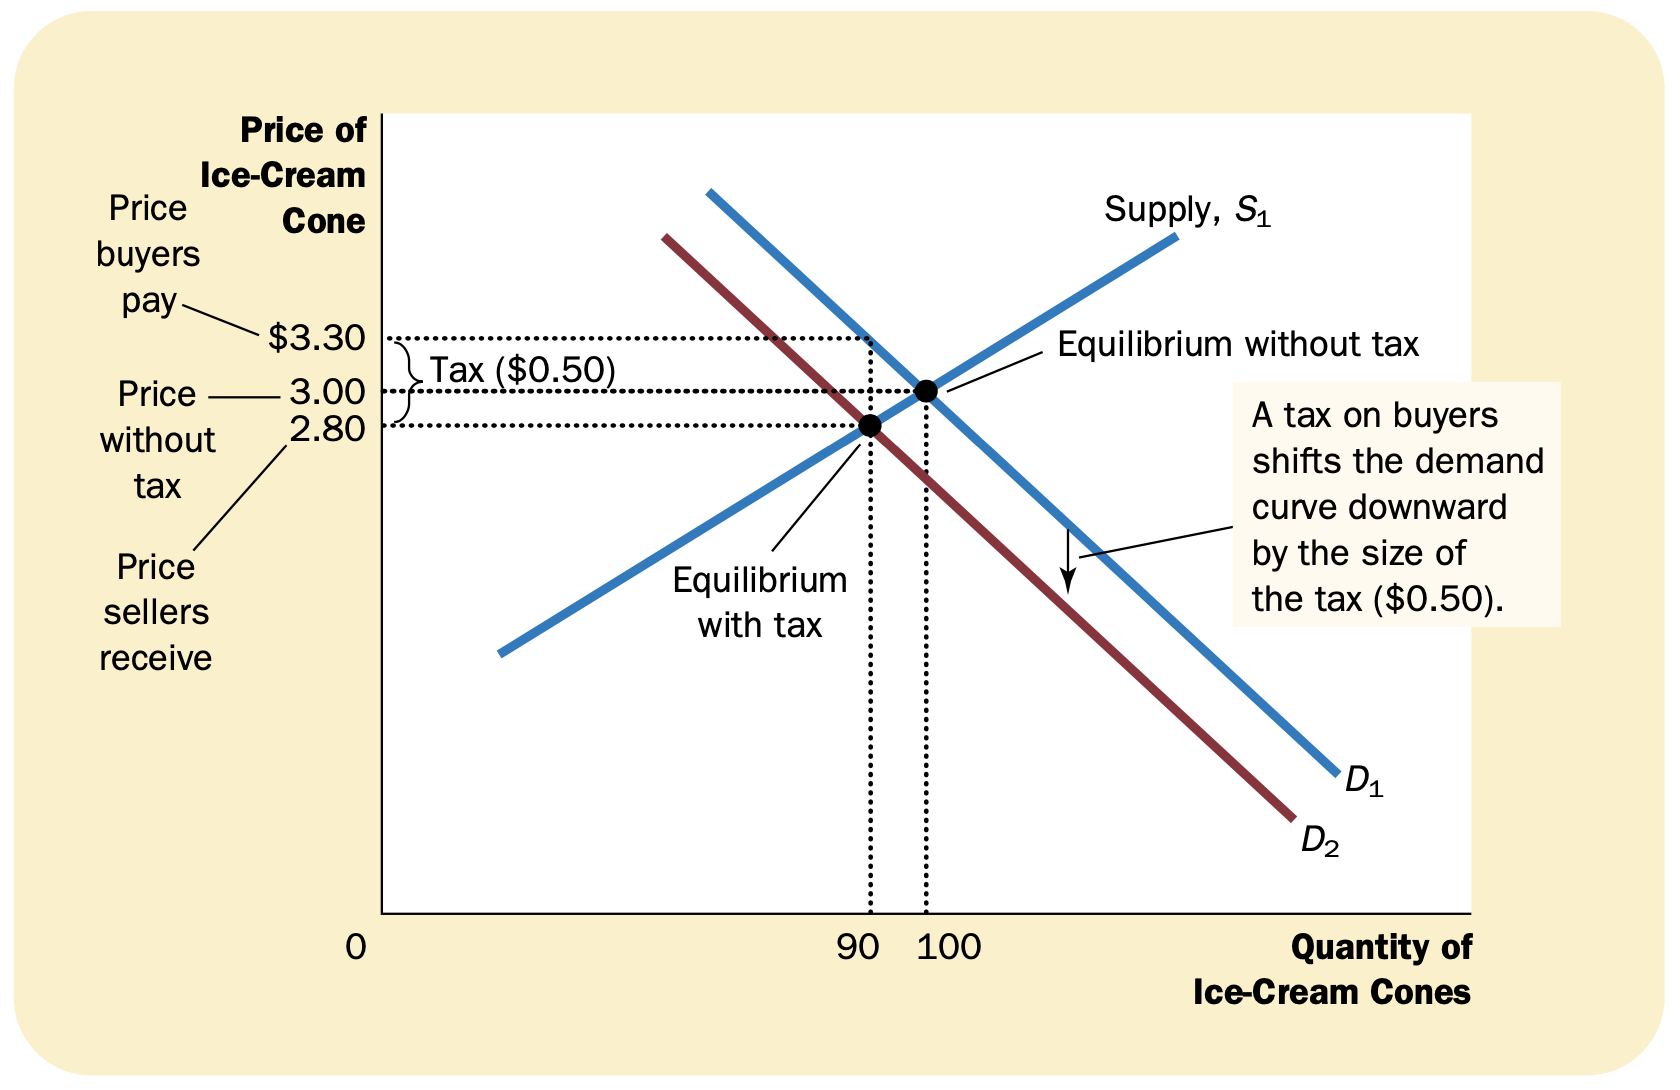
\includegraphics[width=\textwidth]{pics/tax1}
  \caption{向卖者征税}
  \label{fig:tax1}
\end{figure}


结论:
\begin{itemize}
\item 税收抑制了市场活动。当对一种物品征税时,该物品在新均衡时的销售量减少了。
\item 买者与买者分摊了税收负担。新均衡时,买者为该物品支付的更多了,而买者得到更少了。
\end{itemize}




\subsection{向买者征税如何影响市场}


\begin{figure}[!ht]
  \centering
  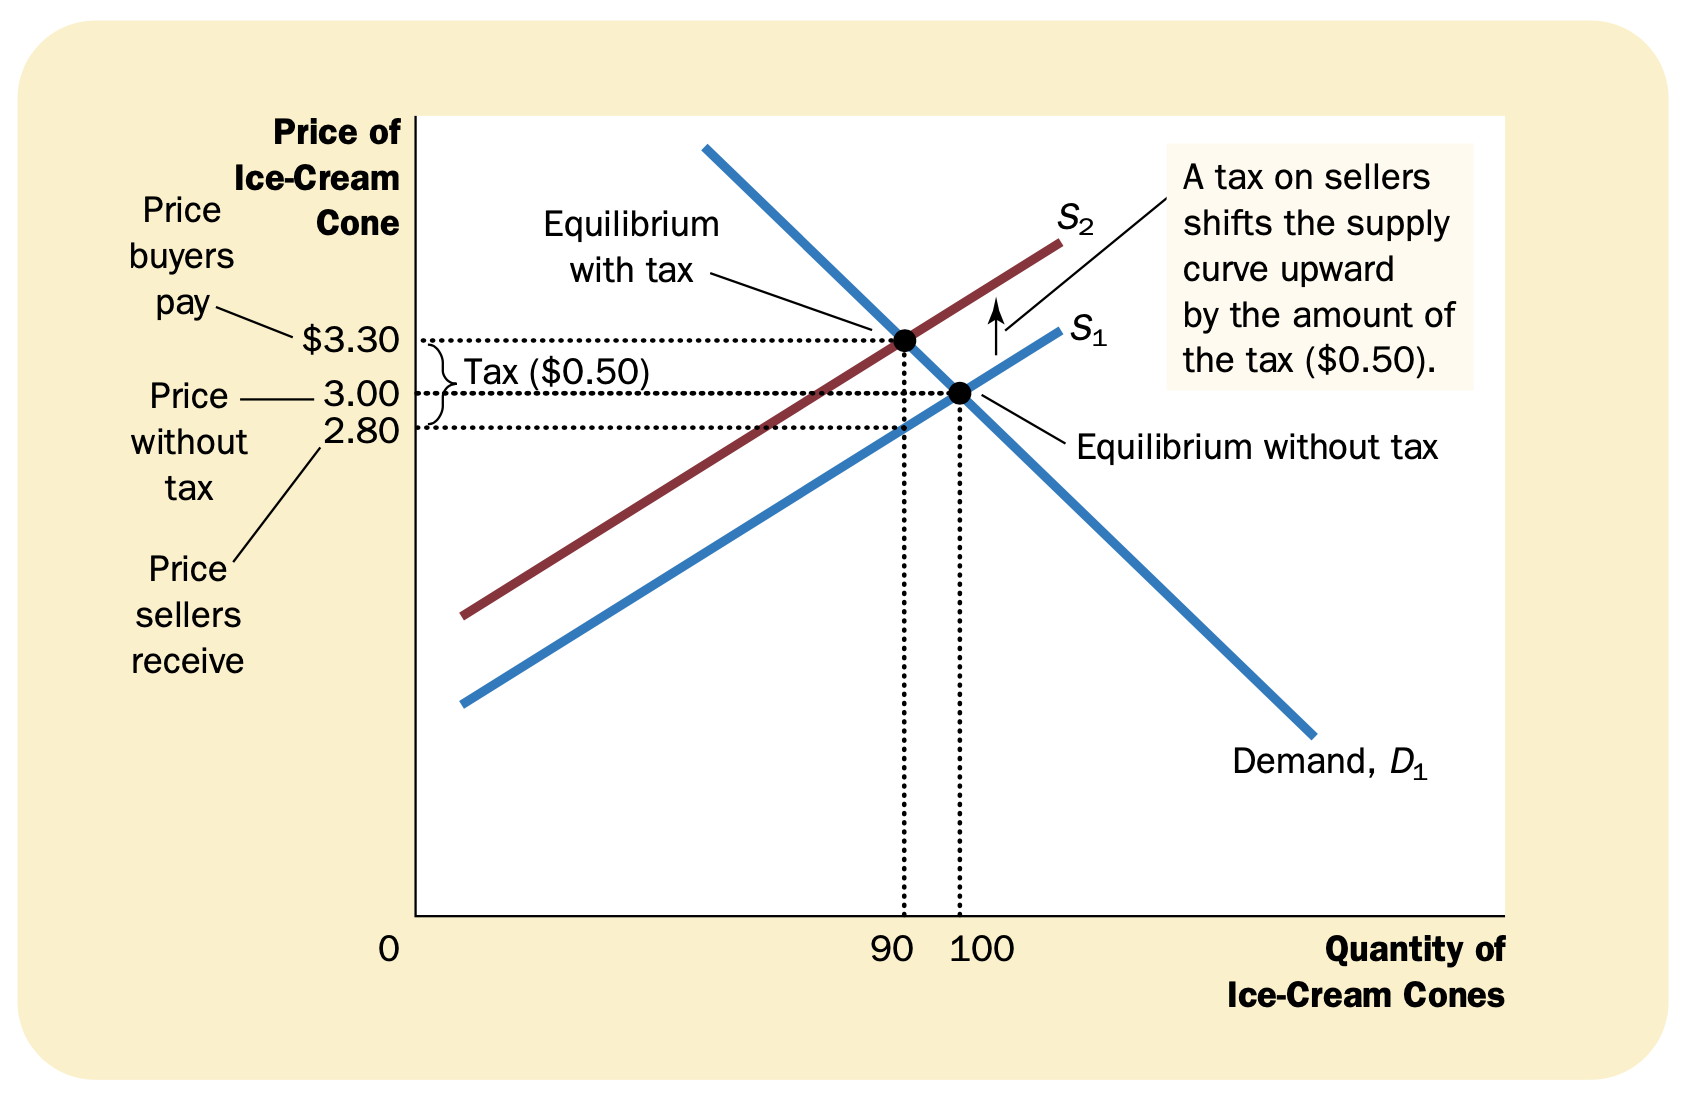
\includegraphics[width=\textwidth]{pics/tax2}
  \caption{向买者征税}
  \label{fig:tax2}
\end{figure}

结论:
对买者征税和对卖者征税是相同的。
对买者征税和对卖者征税的唯一区别是谁来把钱交给政府。




立法者可以决定税收是来自买者的口袋还是来自卖者的口袋,
但他们不能用立法规定税收的真正负担,
税收归宿取决于供给和需求的力量。



